
%% bare_conf.tex
%% V1.4b
%% 2015/08/26
%% by Michael Shell
%% See:
%% http://www.michaelshell.org/
%% for current contact information.
%%
%% This is a skeleton file demonstrating the use of IEEEtran.cls
%% (requires IEEEtran.cls version 1.8b or later) with an IEEE
%% conference paper.
%%
%% Support sites:
%% http://www.michaelshell.org/tex/ieeetran/
%% http://www.ctan.org/pkg/ieeetran
%% and
%% http://www.ieee.org/

%%*************************************************************************
%% Legal Notice:
%% This code is offered as-is without any warranty either expressed or
%% implied; without even the implied warranty of MERCHANTABILITY or
%% FITNESS FOR A PARTICULAR PURPOSE! 
%% User assumes all risk.
%% In no event shall the IEEE or any contributor to this code be liable for
%% any damages or losses, including, but not limited to, incidental,
%% consequential, or any other damages, resulting from the use or misuse
%% of any information contained here.
%%
%% All comments are the opinions of their respective authors and are not
%% necessarily endorsed by the IEEE.
%%
%% This work is distributed under the LaTeX Project Public License (LPPL)
%% ( http://www.latex-project.org/ ) version 1.3, and may be freely used,
%% distributed and modified. A copy of the LPPL, version 1.3, is included
%% in the base LaTeX documentation of all distributions of LaTeX released
%% 2003/12/01 or later.
%% Retain all contribution notices and credits.
%% ** Modified files should be clearly indicated as such, including  **
%% ** renaming them and changing author support contact information. **
%%*************************************************************************
\documentclass[conference]{IEEEtran}

\usepackage{graphicx}
\usepackage{subfigure}
\usepackage{amsmath}
\usepackage{amssymb} 
\usepackage{array}

\usepackage{blindtext}

% Some very useful LaTeX packages include:
% (uncomment the ones you want to load)


% *** MISC UTILITY PACKAGES ***
%
%\usepackage{ifpdf}
% Heiko Oberdiek's ifpdf.sty is very useful if you need conditional
% compilation based on whether the output is pdf or dvi.
% usage:
% \ifpdf
%   % pdf code
% \else
%   % dvi code
% \fi
% The latest version of ifpdf.sty can be obtained from:
% http://www.ctan.org/pkg/ifpdf
% Also, note that IEEEtran.cls V1.7 and later provides a builtin
% \ifCLASSINFOpdf conditional that works the same way.
% When switching from latex to pdflatex and vice-versa, the compiler may
% have to be run twice to clear warning/error messages.






% *** CITATION PACKAGES ***
%
%\usepackage{cite}
% cite.sty was written by Donald Arseneau
% V1.6 and later of IEEEtran pre-defines the format of the cite.sty package
% \cite{} output to follow that of the IEEE. Loading the cite package will
% result in citation numbers being automatically sorted and properly
% "compressed/ranged". e.g., [1], [9], [2], [7], [5], [6] without using
% cite.sty will become [1], [2], [5]--[7], [9] using cite.sty. cite.sty's
% \cite will automatically add leading space, if needed. Use cite.sty's
% noadjust option (cite.sty V3.8 and later) if you want to turn this off
% such as if a citation ever needs to be enclosed in parenthesis.
% cite.sty is already installed on most LaTeX systems. Be sure and use
% version 5.0 (2009-03-20) and later if using hyperref.sty.
% The latest version can be obtained at:
% http://www.ctan.org/pkg/cite
% The documentation is contained in the cite.sty file itself.






% *** GRAPHICS RELATED PACKAGES ***
%
\ifCLASSINFOpdf
  % \usepackage[pdftex]{graphicx}
  % declare the path(s) where your graphic files are
  % \graphicspath{{../pdf/}{../jpeg/}}
  % and their extensions so you won't have to specify these with
  % every instance of \includegraphics
  % \DeclareGraphicsExtensions{.pdf,.jpeg,.png}
\else
  % or other class option (dvipsone, dvipdf, if not using dvips). graphicx
  % will default to the driver specified in the system graphics.cfg if no
  % driver is specified.
  % \usepackage[dvips]{graphicx}
  % declare the path(s) where your graphic files are
  % \graphicspath{{../eps/}}
  % and their extensions so you won't have to specify these with
  % every instance of \includegraphics
  % \DeclareGraphicsExtensions{.eps}
\fi

% *** SPECIALIZED LIST PACKAGES ***
\usepackage{algorithm,algorithmic}





% *** ALIGNMENT PACKAGES ***
%
%\usepackage{array}
% Frank Mittelbach's and David Carlisle's array.sty patches and improves
% the standard LaTeX2e array and tabular environments to provide better
% appearance and additional user controls. As the default LaTeX2e table
% generation code is lacking to the point of almost being broken with
% respect to the quality of the end results, all users are strongly
% advised to use an enhanced (at the very least that provided by array.sty)
% set of table tools. array.sty is already installed on most systems. The
% latest version and documentation can be obtained at:
% http://www.ctan.org/pkg/array


% IEEEtran contains the IEEEeqnarray family of commands that can be used to
% generate multiline equations as well as matrices, tables, etc., of high
% quality.




% *** SUBFIGURE PACKAGES ***
%\ifCLASSOPTIONcompsoc
%  \usepackage[caption=false,font=normalsize,labelfont=sf,textfont=sf]{subfig}
%\else
%  \usepackage[caption=false,font=footnotesize]{subfig}
%\fi
% subfig.sty, written by Steven Douglas Cochran, is the modern replacement
% for subfigure.sty, the latter of which is no longer maintained and is
% incompatible with some LaTeX packages including fixltx2e. However,
% subfig.sty requires and automatically loads Axel Sommerfeldt's caption.sty
% which will override IEEEtran.cls' handling of captions and this will result
% in non-IEEE style figure/table captions. To prevent this problem, be sure
% and invoke subfig.sty's "caption=false" package option (available since
% subfig.sty version 1.3, 2005/06/28) as this is will preserve IEEEtran.cls
% handling of captions.
% Note that the Computer Society format requires a larger sans serif font
% than the serif footnote size font used in traditional IEEE formatting
% and thus the need to invoke different subfig.sty package options depending
% on whether compsoc mode has been enabled.
%
% The latest version and documentation of subfig.sty can be obtained at:
% http://www.ctan.org/pkg/subfig




% *** FLOAT PACKAGES ***
%
%\usepackage{fixltx2e}
% fixltx2e, the successor to the earlier fix2col.sty, was written by
% Frank Mittelbach and David Carlisle. This package corrects a few problems
% in the LaTeX2e kernel, the most notable of which is that in current
% LaTeX2e releases, the ordering of single and double column floats is not
% guaranteed to be preserved. Thus, an unpatched LaTeX2e can allow a
% single column figure to be placed prior to an earlier double column
% figure.
% Be aware that LaTeX2e kernels dated 2015 and later have fixltx2e.sty's
% corrections already built into the system in which case a warning will
% be issued if an attempt is made to load fixltx2e.sty as it is no longer
% needed.
% The latest version and documentation can be found at:
% http://www.ctan.org/pkg/fixltx2e


%\usepackage{stfloats}
% stfloats.sty was written by Sigitas Tolusis. This package gives LaTeX2e
% the ability to do double column floats at the bottom of the page as well
% as the top. (e.g., "\begin{figure*}[!b]" is not normally possible in
% LaTeX2e). It also provides a command:
%\fnbelowfloat
% to enable the placement of footnotes below bottom floats (the standard
% LaTeX2e kernel puts them above bottom floats). This is an invasive package
% which rewrites many portions of the LaTeX2e float routines. It may not work
% with other packages that modify the LaTeX2e float routines. The latest
% version and documentation can be obtained at:
% http://www.ctan.org/pkg/stfloats
% Do not use the stfloats baselinefloat ability as the IEEE does not allow
% \baselineskip to stretch. Authors submitting work to the IEEE should note
% that the IEEE rarely uses double column equations and that authors should try
% to avoid such use. Do not be tempted to use the cuted.sty or midfloat.sty
% packages (also by Sigitas Tolusis) as the IEEE does not format its papers in
% such ways.
% Do not attempt to use stfloats with fixltx2e as they are incompatible.
% Instead, use Morten Hogholm'a dblfloatfix which combines the features
% of both fixltx2e and stfloats:
%
% \usepackage{dblfloatfix}
% The latest version can be found at:
% http://www.ctan.org/pkg/dblfloatfix




% *** PDF, URL AND HYPERLINK PACKAGES ***
\usepackage{url}


\usepackage{mwe}
\usepackage{fancyhdr}
\fancypagestyle{firststyle}
{
    \fancyhf[C]{\fontsize{8}{10} \selectfont \textit{2018 IEEE International Autumn Meeting on Power, Electronics and Computing (ROPEC 2018). Ixtapa, Mexico} }
    \fancyfoot[C]{978-1-5386-5935-9/18/\$31.00 \textcopyright 2018 IEEE}
}




% correct bad hyphenation here
\hyphenation{op-tical net-works semi-conduc-tor}

\renewcommand{\algorithmicrequire}{\textbf{Input:}}
\renewcommand{\algorithmicensure}{\textbf{Output:}}

\begin{document}
%
% paper title
\title{Physics-inspired Algorithm for \\ Bilevel Optimization}


%%%%%%%%%%%%%%%%%%%%%%%%%%%%%%%%%%%%%%%%%%%%%%%%%%%%%%%%%%%%%%%%%%%
% author names and affiliations
%%%%%%%%%%%%%%%%%%%%%%%%%%%%%%%%%%%%%%%%%%%%%%%%%%%%%%%%%%%%%%%%%%%
\author{\IEEEauthorblockN{Jes\'{u}s-Adolfo Mej\'{i}a-de-Dios}
\IEEEauthorblockA{Artificial Intelligence Research Center\\
University of Veracruz\\
Sebasti\'{a}n Camacho 5, Centro \\
Xalapa, Veracruz, 91000, M\'exico\\
Email: jesusmejded@gmail.com}
%%%%%%%%%%%%%%%%%%%%%%%%%%%%%%%%%%%%%%%%%%%%%%%%%%%%%%%%%%%%%%%%%%%%
\and
%%%%%%%%%%%%%%%%%%%%%%%%%%%%%%%%%%%%%%%%%%%%%%%%%%%%%%%%%%%%%%%%%%%%
\IEEEauthorblockN{Efr\'{e}n Mezura-Montes}
\IEEEauthorblockA{Artificial Intelligence Research Center\\
University of Veracruz\\
Sebasti\'{a}n Camacho 5, Centro \\
Xalapa, Veracruz, 91000, M\'exico\\
Email: emezura@uv.mx}
}
%%%%%%%%%%%%%%%%%%%%%%%%%%%%%%%%%%%%%%%%%%%%%%%%%%%%%%%%%%%%%%%%%%%

% make the title area
\maketitle

\thispagestyle{firststyle}
\renewcommand{\headrulewidth}{0in}
\pagestyle{empty}


%\thispagestyle{pageStyleOne}
\pagestyle{fancy}
\chead{\fontsize{8}{10} \selectfont \textit{2018 IEEE International Autumn Meeting on Power, Electronics and Computing (ROPEC 2018). Ixtapa, Mexico} }
\pagenumbering{gobble}



% The abstract
\begin{abstract}
Lorem ipsum dolor sit amet, consectetur adipisicing elit, sed do eiusmod
tempor incididunt ut labore et dolore magna aliqua. Ut enim ad minim veniam,
quis nostrud exercitation ullamco laboris nisi ut aliquip ex ea commodo
consequat. Duis aute irure dolor in reprehenderit in voluptate velit esse
cillum dolore eu fugiat nulla pariatur. Excepteur sint occaecat cupidatat non
proident, sunt in culpa qui officia deserunt mollit anim id est laborum.
\end{abstract}

\IEEEpeerreviewmaketitle


%%%%%%%%%%%%%%%%%%%%%%%%%%%%%%%%%%%%%%%%%%%%%%%%%%%%%%%%%%%%%%%%%%%%%%%%
\section{Introduction}
%%%%%%%%%%%%%%%%%%%%%%%%%%%%%%%%%%%%%%%%%%%%%%%%%%%%%%%%%%%%%%%%%%%%%%%%

An optimization problems can be represented as finding the set:
% 
\begin{align}
    X^* &= \arg \min_{\vec{x} \in X} f(\vec{x}) \\
    &= \{ \vec{x}^* \in X \ : \ f(\vec{x}^*) \leq f( \vec{x} ), \ 
    % 
    \forall
    % 
    \vec{x} \in X \},
    \label{eqn:Xargmin}
\end{align}
% 
where, $X$ is a $D$-dimensional vector space of parameters, usually $X \subset \mathbb{R}^D$
is the domain for $\vec{x}$ representing constraints on allowable values for $\vec{x}$.
Equation \ref{eqn:Xargmin} may be read as: $X^*$ is the set of values (arguments)
$\vec{x} = \vec{x}^*$ that minimize $f(\vec{x})$ subject to $X^*$.

% 
\begin{figure}[!ht]
    \centering
    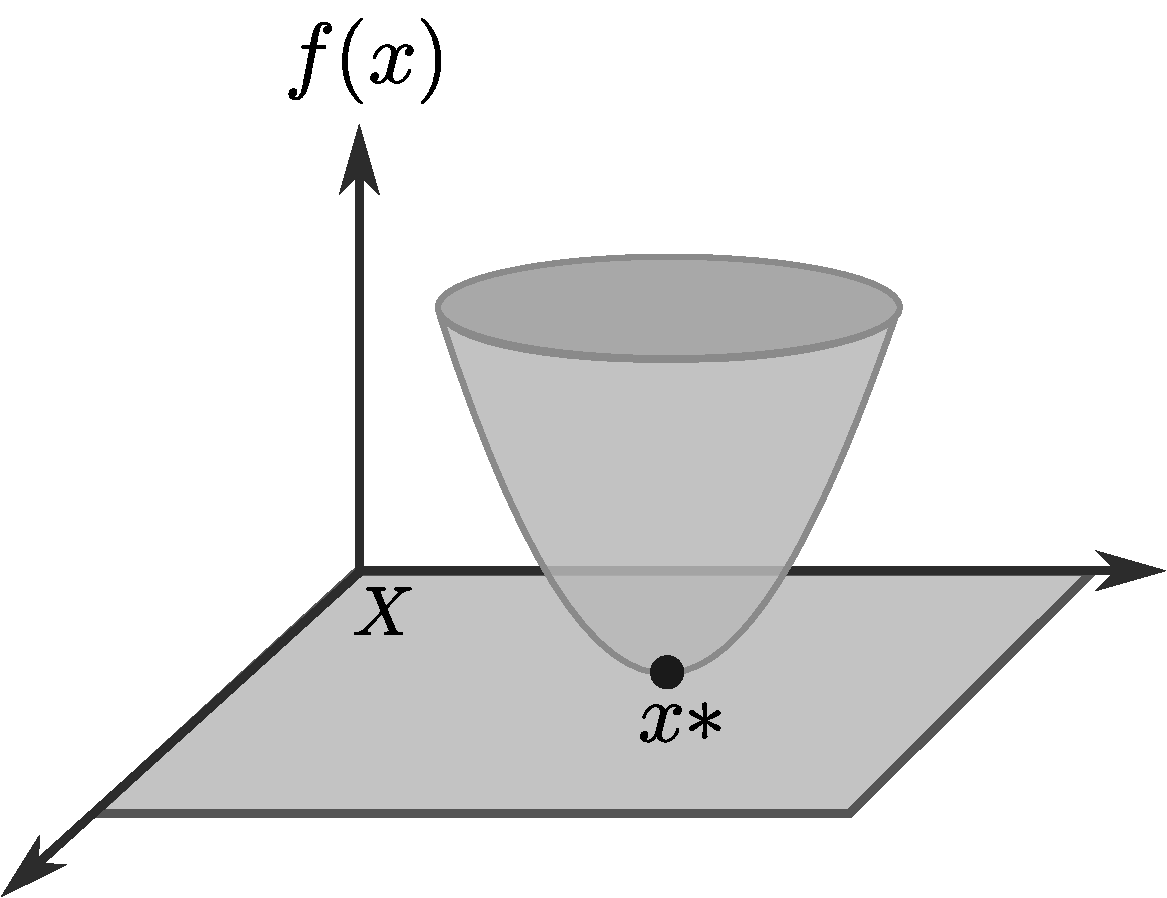
\includegraphics[width=0.5\linewidth]{img/monolevel.pdf}
    \caption{Single-objective optimization problem.}
    \label{fig:single-level}
\end{figure}

An optimization problem is solved only when a global minimum
is found. However, global minimum are, in general, difficult to find. Therefore,
in practice, we often have to find at least a local minimum.

Minimize
\begin{equation}
    F(x,\ y) \ \ x \in X , \ y \in Y 
    \label{eqn:minF1}
\end{equation}
% 
subject to:
% 
\begin{align}
    \label{eqn:y-arg}
    &y \in \arg \min \{ f(x, y) \ : \ g_j(x, y) \leq 0, \ j = 1,\ldots, J \}\\
    &G_k(x, y)  \leq 0, \ k = 1,\ldots,K
    \label{eqn:G}
\end{align}
where $F: X \times Y \to \mathbb{R}$ y $f: X \times Y \to \mathbb{R}$
are the upper-level objective function (leader) and upper-level objective function (follower), respectively. In this work, $X \subseteq \mathbb{R}^n$ and $Y \subseteq \mathbb{R}^m$ is considered. The Figure \ref{fig:bilevel} shows a schematic diagram of a bilevel optimization problem.
% 
\begin{figure}[!ht]
    \centering
    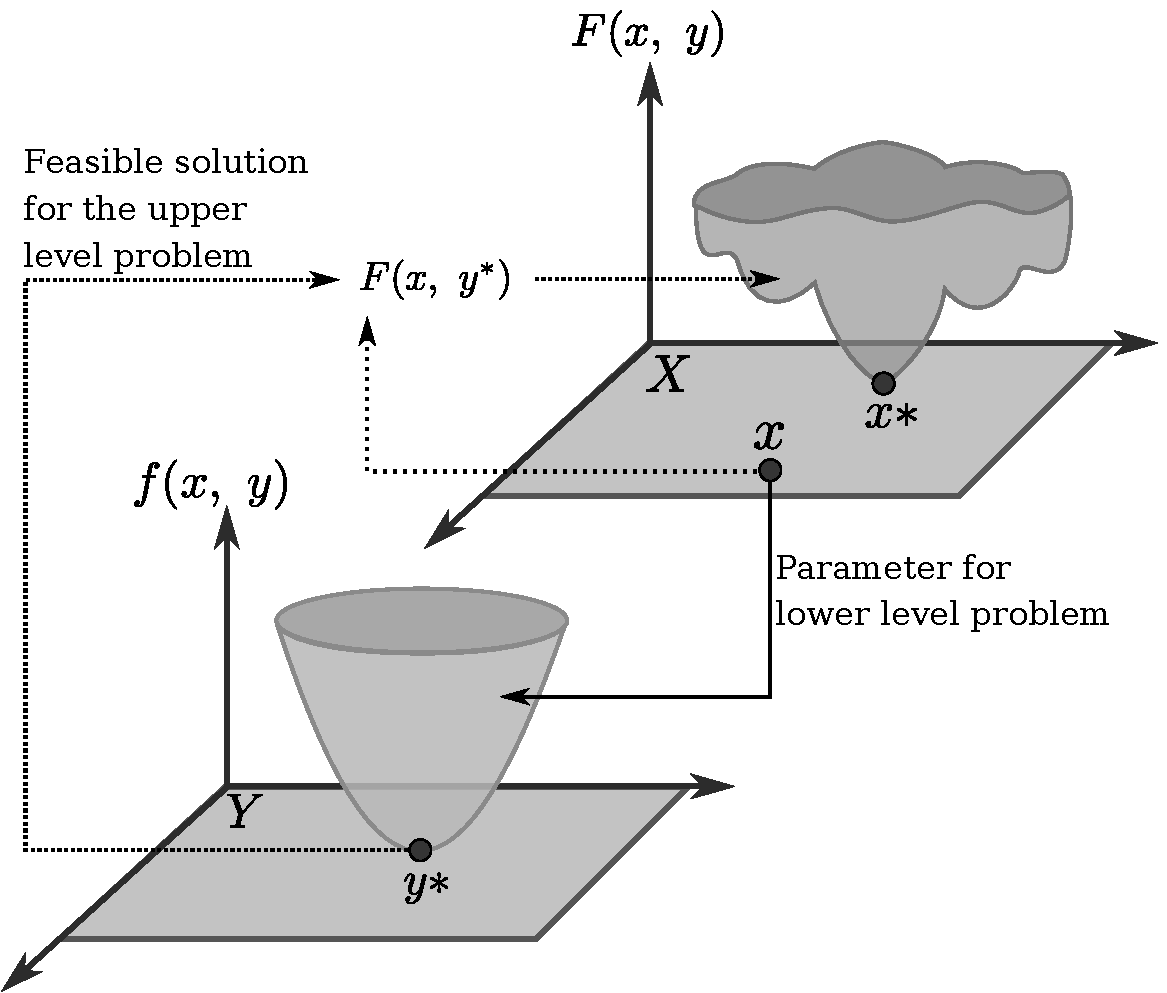
\includegraphics[width=0.8\linewidth]{img/bilevel.pdf}
    \caption{Diagram of a bilevel optimization problem. Here, $y^*$ 
            is defined as in Eq. (\ref{eqn:y-arg}). Note that $(x,\ y^*)$
            is a feasible solution.}
    \label{fig:bilevel}
\end{figure}


%%%%%%%%%%%%%%%%%%%%%%%%%%%%%%%%%%%%%%%%%%%%%%%%%%%%%%%%%%%%%%%%%%%%%%%%
\section{Lower Level Optimizer} % (fold)
%%%%%%%%%%%%%%%%%%%%%%%%%%%%%%%%%%%%%%%%%%%%%%%%%%%%%%%%%%%%%%%%%%%%%%%%
\label{sec:eca}

The center of mass is the unique point $\vec{c}$ at the center of a distribution
of mass $U = \{\vec{u}_1,\; \vec{u}_2 , \ldots , \vec{u}_K \}$ in a space that 
has the property that the weighted sum of position vectors relative to this
point is zero. That is:

\begin{equation}
    \sum_{i = 1}^K m(\vec{u}_i) (\vec{u}_i - \vec{c}) = 0,  \text{ implies } 
    %%%%%%%%%%%%%%%%%%%%%
    \vec{c} = \dfrac{1}{M} \sum_{i = 1}^K  m(\vec{u}_i)  \vec{u}_i,
    \label{eqn:masscenter}
\end{equation}
%
%
where $m(\vec{u}_i)$ is the mass of $\vec{u}_i$ and  $M$ is the sum of the 
masses of vectors in $U$. Here, $m$ is a non-negative function.
 
The lower level optimizer works as follows: for each solution $\vec{y}_i $ in the population $P = \{ \vec{y}_1,\ \vec{y}_2, \ \ldots, \ \vec{y}_{N} \} $
of $N$  solutions, we generate $U_i \subset P $ with $K$ \textbf{different}
solutions such that
% 
$$
\bigcup_{i=1}^N U_i = P.
$$
%
Next, from $U_i$ the center of mass $\vec{c}_i$ is computed by using the Equation \ref{eqn:masscenter} by setting $m(\vec{u}) = f(\vec{x}, \vec{u})$ where $\vec{x}$ is fixed.
After that, \textbf{the worst element} $\vec{u}_{\text{worst}}$ in $U_i$ is selected
according to the following rule:
% 
$$
    \vec{u}_{\text{worst}} \in \arg \min \{f(\vec{x}, \ \vec{u} ) 
    % 
    \ : \
    % 
    \vec{u} \in U_i \}.
$$
% 
Now, we are able to generate a direction to locate a new solution $ \vec{y}_i$
using the already generated center of mass $\vec{c}_i$, $\vec{y}_i$ and $\vec{u}_{\text{worst}}$.
% 
$$
    \vec{h}_i = \vec{y}_i + \eta _{i} ( \vec{c}_i - \vec{u}_{ \text{worst} } ).
$$
% 

To improve the exploration process to avoid premature convergence since ECA can provide a fast convergence. Thus we can take advantage of it to exploit the vicinity near the best solution found using the last objective function evaluations. That is, generating a new solution with Equation \ref{eqn:vcu2}:
%
\begin{equation}
    \vec{h}_i = 
    \begin{cases}
        \vec{y}_i + \eta _{i} ( \vec{c}_i - \vec{u}_{ \text{worst} } ) 
               & \text{ if } t/T < 0.95 \\
        % 
        \vec{y}_i + \eta _{i} ( \vec{y}_{\text{best}} - \vec{c}_i)
               & \text{ otherwise}
    \end{cases}
    \label{eqn:vcu2}
\end{equation}
%
where, $ 0.95$ is the evaluation ratio (current number of function
evaluation / max. number of function evaluations), $t/T$ is the
last percentage of evaluations used for an exploitation process and $\vec{y}_{\text{best}}$
is the best element ever found. Finally, if $\vec{h}_i$  is better than $\vec{y}_i$,
then the worst element in $P$ is replaced by $\vec{h}$.
% 

\begin{algorithm}[!h]
    \caption{ECA pseudocode}
    \label{algoritmoEca}
    \begin{algorithmic}[1]
        \REQUIRE {upper level parameter $\vec{x}$, $K = 7, \; \eta_{\max} = 2$}
        \STATE $N \gets K*D$
        \STATE Initialize a population $P \subset Y$ with $N$ elements
        \WHILE{the end criterion is not achieved}
            \FOR {each $\vec{y}$ in $P$}
                \STATE Generate a subset $U \subset P$ with $K$ solutions
                \STATE Calculate $\vec{c}$ using $U$ with (\ref{eqn:masscenter})
                \STATE $\eta \gets \text{rand}(0,\; \eta_{\max}) $ 
                \STATE Compute $\vec{h}$ using Eq. (\ref{eqn:vcu2})
                % 
                \IF{$ f (\vec{x},\ \vec{y}) < f (\vec{x}, \ \vec{h})  $}
                    \STATE Replace worst element in $P$ with $\vec{h}$
                \ENDIF
                % 
            \ENDFOR
            % 
            \STATE Resize $P$ if necessary.
        \ENDWHILE
        \RETURN {the best solution in $P$}
    \end{algorithmic}
\end{algorithm}

Optionally, a linear reduction of the population (deleting the worst elements) can
be applied. The initial population size is $ N(0) = K*D$ and the final population
size $N(T) =  2*K$ (for successfully generating the center of mass). Thus, the
population size over time is:
\begin{align}
    N(t) &= KD - \dfrac{(KD - 2K)  t}{T} \\ \nonumber
         &= K \left( D - \dfrac{(D - 2)  t}{T} \right),
\end{align}
% 
where $t = 0,1,2,\ldots,T$ and $T$ is the maximum number of iterations.


% section eca (end)

\section{BCA} % (fold)
\label{sec:bca}

The variation operator of BCA is considering some properties, first
the population for bilevel optimization is defined as follows: 
$$
    P = \{ (\vec{x}_1,\; \vec{y}_1), \ (\vec{x}_2,\; \vec{y}_2), \ldots,
           (\vec{x}_N,\; \vec{y}_N)
         \}
         \subset X \times Y .
$$
% 
Let $F$ and $f$ be defined as in (\ref{eqn:minF1})-(\ref{eqn:G}), and without lost 
of generality, we can assume that both $F$ and $f$ are  non-negative and we want to maximize them. For each iteration and each $(\vec{x}_i,\; \vec{y}_i) \in P$, a new solution is generated using the following formulation:
% 
\begin{equation}
    \vec{p}_i = 
    \begin{cases}
        \vec{x}_i + \eta _{i} ( \vec{c}_i - \vec{u}_{ \text{worst} } ) 
               & \text{ if } t/T < 0.95 \\
        % 
        \vec{x}_i + \eta _{i} ( x_{\text{best}} - \vec{c}_i)
               & \text{ otherwise}
    \end{cases}
    \label{eqn:vcu2F}
\end{equation}
% 
%
where the $\vec{c}_i$ is the center of mass is computed using:
%
\begin{equation}
    \vec{c}_i = \dfrac{1} {W} \sum_{(x,y) \in U} F(\vec{x},\ \vec{y}) \cdot \vec{x} , 
            \hspace{0.5cm} 
            W = \sum_{ (x,y) \in U} F(\vec{x},\ \vec{y}),
            % \hspace{0.5cm} 
            % U \subseteq P.
    \label{eqn:centerF}
\end{equation} 
% 
with $U \subset P $ such that card$(U) = K$  and $\vec{u}_{ \text{worst}}$ is the first coordinate of the worst element in $U$.

Finally, the new solution is given by $ (\vec{p}, \ \vec{q}) $ which may 
replace the worst solution in $ P $. Here,
$  \vec{q} = \arg \min _ {\vec{z} \in Y} f (\vec{p}, \ \vec{z}) $ obtained
by applying ECA. This procedure is summarized in Algorithm \ref{alg:BCA}.

Note that the nested case was considered. Experiments are currently being carried out in test functions to know the efficiency of BCA and how it is positioned with respect to algorithms of the state of the art.
% 

Algorithm \ref{alg:BCA} is the general pseudocode of ECA.

\begin{algorithm}[!t]
    \caption{BCA pseudocode}
    \label{alg:BCA}
    \begin{algorithmic}[1]
        % \Procedure{BCA}{$K = 7, \; \eta_{\max} = 2,\ t/T = 0.95,\ P_{\text{bin}} = 0.7$}
        \STATE $N \gets K * D$
        \STATE Generate and evaluate start population $P$ with $N$ elements
        \WHILE{the end criterion is not achieved}
            \FOR {each $(\vec{x},\; \vec{y})$ in $P$}
                \STATE Generate a subset $U \subset P$ such that  card$(U) = K$
                \STATE Calculate $\vec{c}$ using $U$ with (\ref{eqn:centerF})
                \STATE $\eta \gets \text{rand}(0,\; \eta_{\max}) $ 
                \STATE Calculate $\vec{p}$ using Eq. (\ref{eqn:vcu2F})
                \STATE Find $\displaystyle \vec{q} \in \arg \min_{\vec{z}\in Y} f(\vec{p},\ \vec{z})$ by using ECA
                
                \IF{$ F (\vec{x},\ \vec{y}) < F (\vec{p},\ \vec{q})  $}
                    \STATE Replace worst element in $P$ with $(\vec{p},\ \vec{q})$.
                \ENDIF
            \ENDFOR
        \ENDWHILE
        \STATE Report best solution in $P$
        % \EndProcedure
    \end{algorithmic}
\end{algorithm}

\section{Experiments and Discussion}


The algorithm BCA for bilevel optimization. BCA is used to solve the test functions
described in \cite{sinha2012unconstrained,sinha2014test}.

\begin{itemize}
    \item Upper level dimension $D_{UL} = 5$
    \item Lower level dimension $D_{LL} = 5$
\end{itemize}

Function Evaluations (FE) were fixed for the upper level ($500D_{UL} = 2500$) and
the lower level ($500D_{UL}*500D_{LL} = 6,250,000$).



\begin{table}[!t]
\renewcommand{\arraystretch}{1.3}
    \caption{Leader accuracy statistics obtained from 31 independent runs.}
    \label{tab:leader}
    \centering
    \begin{tabular}{|c|c|c|c|c|c|c|}
%---------------------------------------------
\hline
&\textbf{Best}&\textbf{Median}&\textbf{Mean}&\textbf{Worst}&\textbf{Std.}\\ \hline 
%---------------------------------------------
\textbf{SMD1} & 1.51E--05 & 5.35E--05 & 5.28E--05 & 8.34E--05 & 1.90E--05 \\ \hline 
\textbf{SMD2} & 1.50E--05 & 4.68E--05 & 5.88E--05 & 3.11E--04 & 5.13E--05 \\ \hline 
\textbf{SMD3} & 1.57E--05 & 5.51E--05 & 2.40E--04 & 3.54E--03 & 6.60E--04 \\ \hline 
\textbf{SMD4} & 4.09E--08 & 4.90E--05 & 6.20E--05 & 3.01E--04 & 6.70E--05 \\ \hline 
\textbf{SMD5} & 2.30E--05 & 5.03E--05 & 4.78E--05 & 8.33E--05 & 1.74E--05 \\ \hline 
\textbf{SMD6} & 1.57E--01 &  1.90E+01 &  2.59E+01 &  1.40E+02 &  2.95E+01 \\ \hline 
\textbf{SMD7} & 9.34E--01 & 9.75E--01 &  1.19E+00 &  3.81E+00 & 6.00E--01 \\ \hline 
\textbf{SMD8} & 1.58E--05 & 6.49E--05 & 1.83E--04 & 2.23E--03 & 4.11E--04 \\ \hline 
%---------------------------------------------
    \end{tabular}
\end{table}

\begin{table}[!t]
\renewcommand{\arraystretch}{1.3}
    \caption{Follower accuracy statistics obtained from 31 independent runs.}
    \label{tab:follower}
    \centering
    \begin{tabular}{|c|c|c|c|c|c|c|}
%---------------------------------------------
\hline
&\textbf{Best}&\textbf{Median}&\textbf{Mean}&\textbf{Worst}&\textbf{Std.}\\ \hline 
%---------------------------------------------
\textbf{SMD1} & 2.67E--06 & 2.06E--05 & 2.14E--05 & 4.75E--05 & 9.77E--06 \\ \hline 
\textbf{SMD2} & 3.56E--06 & 1.81E--05 & 2.07E--05 & 4.60E--05 & 1.15E--05 \\ \hline 
\textbf{SMD3} & 1.87E--07 & 2.24E--05 & 3.12E--04 & 4.31E--03 & 9.28E--04 \\ \hline 
\textbf{SMD4} & 6.23E--06 & 3.65E--05 & 1.53E--04 & 7.96E--04 & 2.33E--04 \\ \hline 
\textbf{SMD5} & 2.50E--06 & 2.01E--05 & 2.19E--05 & 4.55E--05 & 1.28E--05 \\ \hline 
\textbf{SMD6} & 3.91E--04 & 2.86E--02 & 4.23E--02 & 1.84E--01 & 4.35E--02 \\ \hline 
\textbf{SMD7} &  3.71E+02 &  3.74E+02 &  3.74E+02 &  3.75E+02 &  1.01E+00 \\ \hline 
\textbf{SMD8} & 1.18E--06 & 2.33E--05 & 6.53E--05 & 7.93E--04 & 1.44E--04 \\ \hline 

%---------------------------------------------
    \end{tabular}
\end{table}

\begin{table}[!t]
\renewcommand{\arraystretch}{1.3}
    \caption{leader evals statistics obtained from 31 independent runs.}
    \label{tab:follower}
    \centering
    \begin{tabular}{|c|c|c|c|c|c|c|}
%---------------------------------------------
\hline
&\textbf{Best}&\textbf{Median}&\textbf{Mean}&\textbf{Worst}&\textbf{Std.}\\ \hline 
%---------------------------------------------
\textbf{SMD1} & 1244 & 1526 & 1539.42 & 1879 & 152.119 \\ \hline
\textbf{SMD2} & 1244 & 1481 & 1482.84 & 2501 & 220.7   \\ \hline
\textbf{SMD3} & 1365 & 1526 & 1647.84 & 2501 & 287.517 \\ \hline
\textbf{SMD4} & 1169 & 1435 & 1437.26 & 1800 & 131.393 \\ \hline
\textbf{SMD5} & 1317 & 1526 & 1554.42 & 1898 & 137.766 \\ \hline
\textbf{SMD6} & 2501 & 2501 & 2501 &  2501 &   0   \\ \hline
\textbf{SMD7} & 2501 & 2501 & 2501 &  2501 &   0   \\ \hline
\textbf{SMD8} & 1780 & 2219 & 2234.65 & 2501 & 206.959 \\ \hline


%---------------------------------------------
    \end{tabular}
\end{table}

\begin{table}[!t]
\renewcommand{\arraystretch}{1.3}
    \caption{follower evals statistics obtained from 31 independent runs.}
    \label{tab:follower}
    \centering
    \begin{tabular}{|c|c|c|c|c|c|c|}
%---------------------------------------------
\hline
&\textbf{Best}&\textbf{Median}&\textbf{Mean}&\textbf{Worst}&\textbf{Std.}\\ \hline 
%---------------------------------------------
\textbf{DMD1} & 3110000  & 3815000  & 3848548.4  & 4697500  & 380298.6 \\ \hline
\textbf{DMD2} & 3110000  & 3702500  & 3707096.8  & 6252500  & 551750.7 \\ \hline
\textbf{DMD3} & 3412500  & 3815000  & 4119596.8  & 6252500  & 718793.3 \\ \hline
\textbf{DMD4} & 2922500  & 3587500  & 3593145.2  & 4500000  & 328481.3 \\ \hline
\textbf{DMD5} & 3292500  & 3815000  & 3886048.4  & 4745000  & 344415.4 \\ \hline
\textbf{DMD6} & 6252500  & 6252500  & 6252500  & 6252500  & 0 \\ \hline
\textbf{DMD7} & 6252500  & 6252500  & 6252500  & 6252500  & 0 \\ \hline
\textbf{DMD8} & 4450000  & 5547500  & 5586612.9  & 6252500  & 517397.6 \\ \hline
%---------------------------------------------
    \end{tabular}
\end{table}

% %%%%%%%%%%%%%%%%%%%%%%%%%%%%%%%%%%%%%%%%%%%%%%%%%%%%%
% %%%%%%%%%%%%%%%%%%%%%%%%%%%%%%%%%%%%%%%%%%%%%%%%%%%%%

\begin{table}[!t]
\renewcommand{\arraystretch}{1.3}
    \caption{Function values at median BCA and BLEAQ obtained from 31 independent runs.}
    \label{tab:leader2}
    \centering
    \begin{tabular}{|c|c|c||c|c|}
%---------------------------------------------
\hline
& \multicolumn{2}{c||}{Upper Level} & \multicolumn{2}{c|}{Lower Level} \\ \hline
& BCA & BLEAQ & BCA & BLEAQ \\ \hline
%---------------------------------------------
 % & bca.ul & bleaq.ul & bca.ll & bleaq.ll \\ \hline
SMD1 & \textbf{1526} & 1600 & 3815000 & \textbf{116088} \\ \hline
SMD2 & \textbf{1481} & 1925 & 3702500 & \textbf{113504} \\ \hline
SMD3 & \textbf{1526} & 1630 & 3815000 & \textbf{122542} \\ \hline
SMD4 & \textbf{1435} & 1750 & 3587500 & \textbf{70906} \\ \hline
SMD5 & \textbf{1526} & 3031 & 3815000 & \textbf{147289} \\ \hline
SMD6 &     2501      & \textbf{1016} & 6252500 & \textbf{7055} \\ \hline
SMD7 &     2501      & \textbf{2104} & 6252500 & \textbf{130195} \\ \hline
SMD8 & \textbf{2219} & 5569 & 5547500 & \textbf{289886} \\ \hline
%---------------------------------------------
    \end{tabular}
\end{table}

% %%%%%%%%%%%%%%%%%%%%%%%%%%%%%%%%%%%%%%%%%%%%%%%%%%%%%
\begin{table}[!t]
\renewcommand{\arraystretch}{1.3}
    \caption{Evals median BCA and BLEAQ obtained from 31 independent runs.}
    \label{tab:leader2}
    \centering
    \begin{tabular}{|c|c|c||c|c|}
%---------------------------------------------
\hline
& \multicolumn{2}{c||}{Upper Level} & \multicolumn{2}{c|}{Lower Level} \\ \hline
& BCA & BLEAQ & BCA & BLEAQ \\ \hline
%---------------------------------------------
SMD1  & 5.36E--05 & 9.91E--05 & 2.07E--05 & 6.72E--05 \\ \hline
SMD2  & 4.68E--05 & 2.82E--04 & 1.82E--05 & 3.84E--04 \\ \hline
SMD3  & 5.51E--05 & 4.96E--06 & 2.25E--05 & 6.26E--06 \\ \hline
SMD4  & 4.90E--05 & 1.54E--04 & 3.66E--05 & 6.12E--04 \\ \hline
SMD5  & 5.04E--05 & 1.62E--04 & 2.01E--05 & 3.08E--04 \\ \hline
SMD6  &  1.90E+01 & 1.46E--13 & 2.87E--02 & 8.66E--16 \\ \hline
SMD7  & 9.76E--01 & 9.76E--02 &  3.75E+02 &  1.25E+02 \\ \hline
SMD8  & 6.50E--05 & 7.46E--03 & 2.33E--05 & 5.63E--03 \\ \hline

%---------------------------------------------
    \end{tabular}
\end{table}

\section{Conclusions}
The conclusion goes here.


\section*{Acknowledgment}


The authors would like to thank...\cite{deb2000efficient}





% trigger a \newpage just before the given reference
% number - used to balance the columns on the last page
% adjust value as needed - may need to be readjusted if
% the document is modified later
%\IEEEtriggeratref{8}
% The "triggered" command can be changed if desired:
%\IEEEtriggercmd{\enlargethispage{-5in}}

\bibliographystyle{IEEEtran}
\bibliography{IEEEabrv,../../../conf/references,../../../conf/references-bilevel}



% that's all folks
\end{document}


